\chapter{Projekt systemu}
\thispagestyle{chapterBeginStyle}

    W tej części opisane zostały wymagania dla aplikacji w kontekście możliwości interakcji przez
użytkownika.



\section{Wymagania aplikacji}
    W ramach stworzonej aplikacji, użytkownik ma możliwość:
\begin{enumerate}
    \item wybrać jedną z predefiniowanych paczek łamigłówek, by przejść do wyboru łamigłówki
    \item wybrać jedną z predefiniowanych łamigłówek w paczce, by przejść do jej rozwiązywania
    \item rozwiązać łamigłówkę przy użyciu wyświetlanej planszy
    \item oznaczać pola, co do których ma pewność, że są puste
    \item zobaczyć stan łamigłówki w menu wyboru, by mógł ocenić:
    \begin{itemize}
        \item czy łamigłówka została rozpoczęta,
        \item czy łamigłówka została ukończona bez przegranej,
        \item czy łamigłówka została ukończona z przegraną.
    \end{itemize}
    \item wprowadzić łamigłówkę dla solvera za pomocą ekranu wprowadzania łamigłówki
    \item wybrać łamigłówkę do rozwiązania dla solvera
    \item nakazać rozwiązanie wprowadzonej łamigłówki
\end{enumerate}

    Oprócz tego, aplikacja:
\begin{enumerate}
    \item śledzi błędy użytkownika w trakcie rozwiązywania łamigłówki i przerywa jej rozwiązywanie
w przypadku popełnienia zbyt wielu błędów
    \item zapisuje postęp rozwiązywania łamigłówki przy wyjściu do poprzedniego ekranu
\end{enumerate}



\section{Nawigacja pomiędzy aktywnościami}
    Aplikacja otwiera się w menu głównym. W menu głównym dostępne są dwie zakładki: zakłada użytkownika
i zakładka w solvera. W zakładce użytkownika użytkownik najpierw wybiera paczkę łamigłówek, a
następnie łamigłówkę do rozwiązania, po czym przechodzi do ekranu rozwiązywania. W zakładce solvera
dostępna jest lista wprowadzonych i predefiniowanych łamigłówek dla solvera. Użytkownik może przejść
do ekranu wprowadzania łamigłówki - by dodać kolejną łamigłówkę - bądź do ekranu automatycznego rozwiązywania,
gdzie nakazuje solverowi rozwiązanie wprowadzonej łamigłówki.

    Zależności między opisanymi aktywnościami są ukazane na diagramie.

\begin{figure}[!htb]
    \centering
    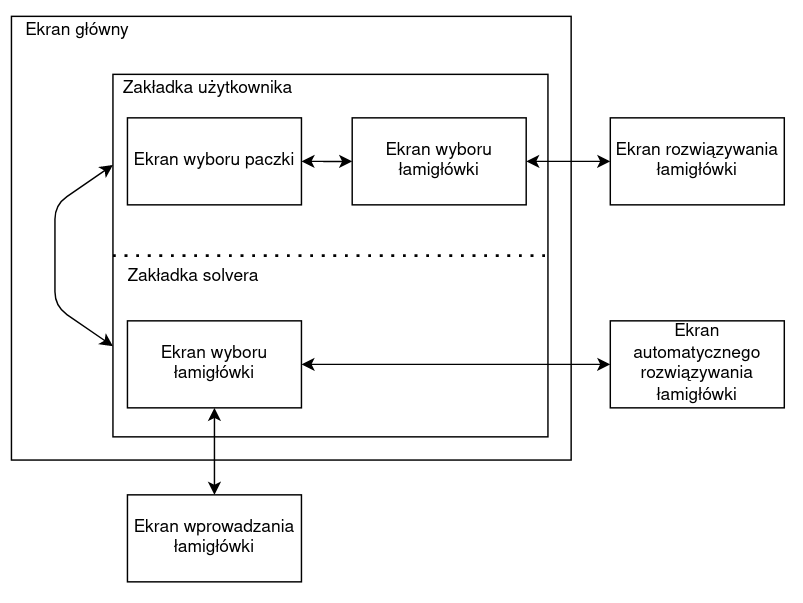
\includegraphics[width=\textwidth]{images/screens_diagram.png}
    \caption{Diagram zależności między aktywnościami}
    \label{diagAktywnosci}
\end{figure}
